\subsection{Disponibilidad}
    
As we mentioned in the introduction to this chapter, the data sets may be available in the original source, but not by
This means that they are accessible.
The challenges that we encounter with the raw data, direct from the source of origin, are the following: \\   
 
\textbf{Location}. Data sets are available in organized open data portals
and structured, you usually need a search and selection task
sometimes complicated. Although companies put more and more of their part in offering an interface
pleasant and functional to users, this task requires a research work by the user,
Since possibly, you should look in different portals. \\

\textbf{Extraction}. Data sets are usually available through a programming interface
of applications (API) not easily interpretable by the average user. Normally has
a document that describes each of the fields and values that are presented in the document and how to use the API. \\

\textbf{Readability}. Usually the data sets are represented in a format to be processed by
some software, so its reading is complicated by the average user, at best,
they will be represented in a table and even then, it will be very difficult to extract information.

Therefore, we can not say that these data are accessible in a useful way for the average user. \\

\subsubsection{How to solve it.} 

We must provide the information required by the user directly, easy to read and interpret. In a format
that is easy and fast to assimilate.

For the correct use of the data we will have to carry out processes such as extraction, transformation and
data cleaning, so you get the data you need to show the useful information.
 
\subsubsection{How we solve it. Aire Guru.} 

Our tool uses the air quality data provided by the city of Malaga in its open data portal.\footnote{\url{https://datosabiertos.malaga.eu/}}\\
\begin{figure}[ht]
    \centering
   \subfigure[Main page]
    {\includegraphics[width=5.5cm  ]{OpenDataPortal}}
    \hfill
    \subfigure [Category environment]
       { 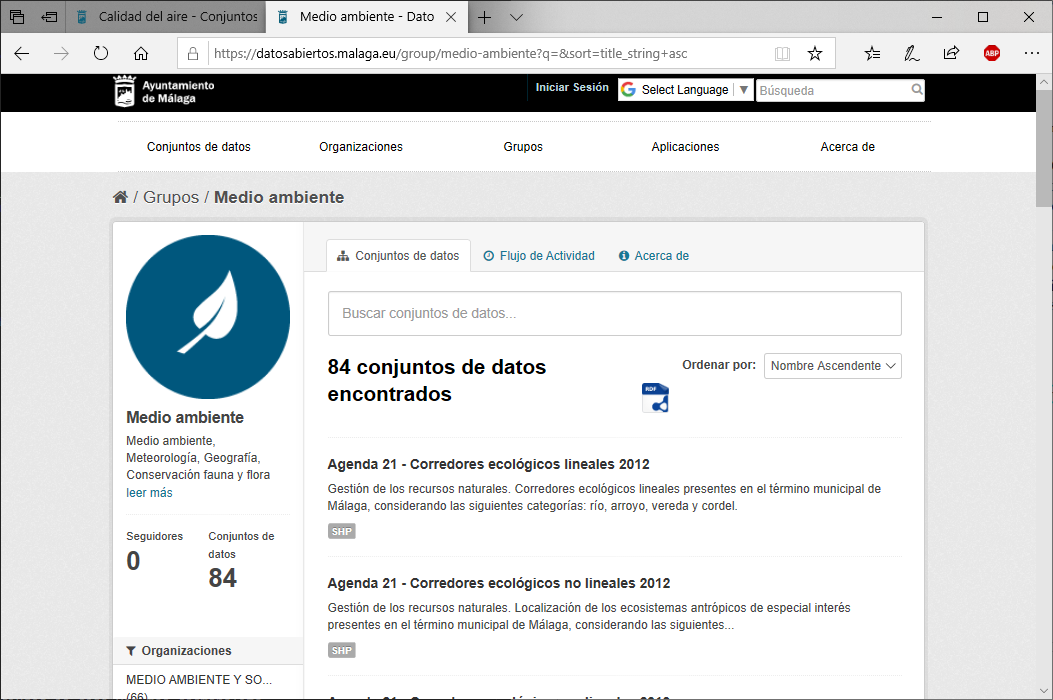
\includegraphics[width=5.5cm]{openDataPortalEnviromentCategory}}
    \vfill
     \subfigure[GeoJson Document]
     { \centering 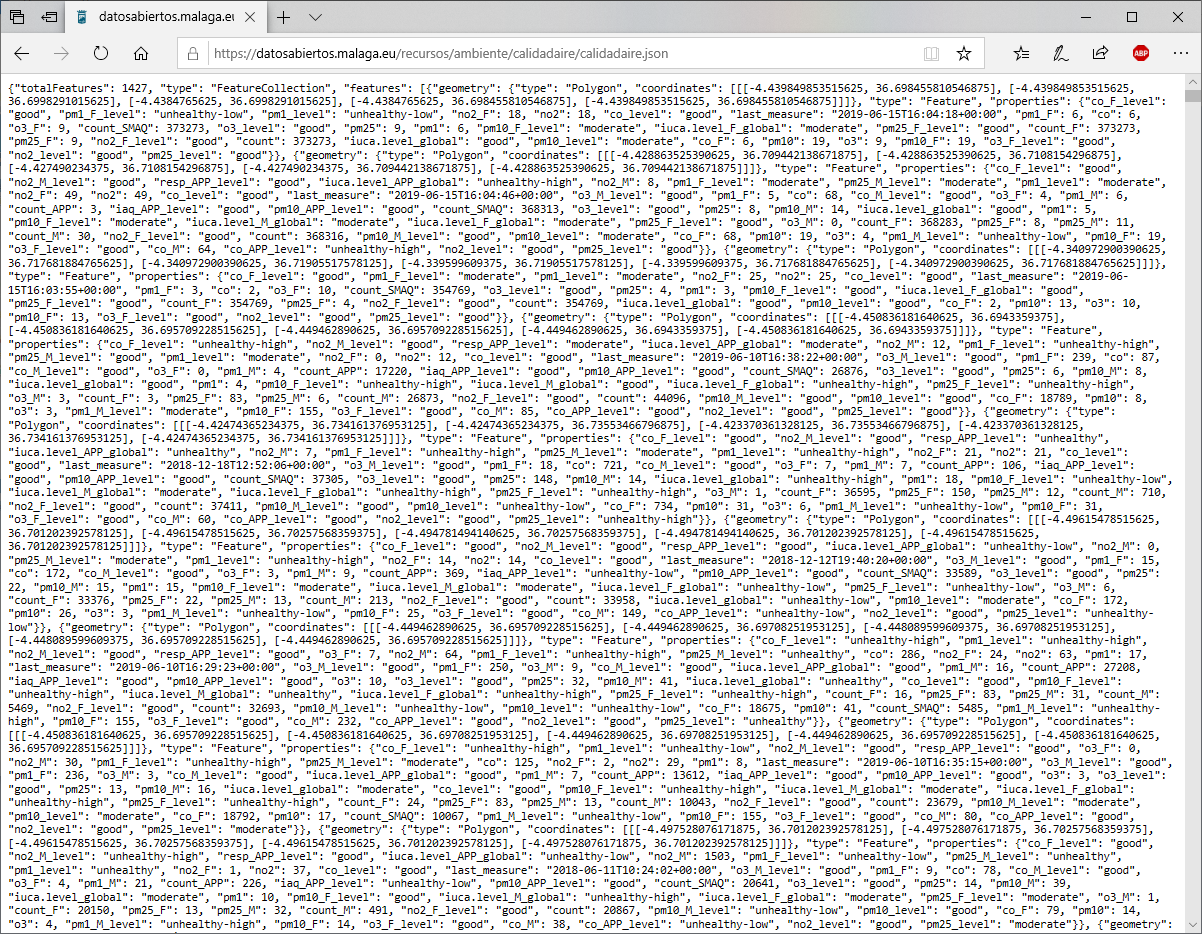
\includegraphics[width=4.75cm]{geoJsonAirQualityDataRaw}}
  
  \caption{Open Data Portal Malaga}
    \end{figure}

    This data portal offers an offer of categories represented by icons, so it is necessary to know in which category the set is classified
    of data, once the category is accessed, we have a search bar that allows us to insert the keywords to search the data set
    wanted.\\
    
    In this case you can click on the link and this will open the data in a new tab, so the use of a computer system
    for downloading the data is not strictly necessary, but we can see that the format is not readable, at least from the point
    of human sight.

AireGuru \footnote{\url{https:\\aire.guru}} offers all the necessary information on a web platform with an adapted visualization
to human understanding.
\newpage
\elsparagraph{Evaluation}  

\begin{itemize}
    \done Location. The location of the data is direct, since it offers information from the first moment in which the web is accessed. On the main page
         presents the levels of pollution in all areas without the need to make any selection.
    \done Extraction. No software or computer knowledge is necessary to access the information.
    \done Readability. It contains a map where the pollution levels are presented by colors. These colors are defined by a fair legend
         below the map. It has a glossary that explains the concepts presented on the website, the meaning of each section and how
         browse the web page.
 

\end{itemize}
\newpage

 


